% !TEX root = main.tex
\renewcommand{\labelenumi}{\alph{enumi})}

\section*{Examen 1}

\begin{questions}
\question A partir del siguiente autómata $M_{1}$, mostrado como tabla de transiciones: \\
    \begin{tabular}{|p{3cm}||p{3cm}|p{3cm}|p{3cm}|p{3cm}|}
        \hline
        \multicolumn{5}{|c|}{Tabla de transiciones} \\
        \hline
        & Q&0&1&2\\
        \hline
        i   & $q_{0}$    &$q_{0}$&   $q_{1}$ &   $q_{2}$ \\
        &   $q_{1}$  & $q_{3}$   &$q_{1}$ &   $q_{2}$\\
        f &$q_{2}$ & $q_{3}$&  $q_{3}$ &   $q_{2}$\\
        &$q_{3}$& $q_{3}$&  $q_{3}$ &   $q_{3}$\\
        \hline
   \end{tabular}
   \begin{enumerate}
        \item Describe el lenguaje $L_{1}$ que corresponde a L($M_{1}$)
        y da la definici\'on completa de la tupla que define al aut\'omata.
            \begin{solution}
                $L_{1} = \{ w \in \Sigma ^{*} | w = 0^{a}1^{a}2^{b}\}$ donde $a \in \mathbb N$ y $b \in \mathbb Z ^{+}\}$

                $Q = \{q_{0},q_{1},q_{2},q_{3}\}$

                $\Sigma = \{0,1,2\}$

                $q_{0} \in Q$ Es el estado inicial

                $F \subseteq Q$ 

                $F = {q_{2}}$ 

                Funci\'iones de transici\'on:

                $\delta (q_{0}, 0) = q_{0}$

                $\delta (q_{0}, 1) = q_{1}$

                $\delta (q_{0}, 2) = q_{2}$

                $\delta (q_{1}, 0) = q_{3}$

                $\delta (q_{1}, 1) = q_{1}$

                $\delta (q_{1}, 2) = q_{2}$

                $\delta (q_{2}, 0) = q_{3}$

                $\delta (q_{2}, 1) = q_{3}$

                $\delta (q_{2}, 2) = q_{2}$

                $\delta (q_{3}, 0) = q_{3}$

                $\delta (q_{3}, 1) = q_{3}$

                $\delta (q_{3}, 2) = q_{3}$    
            \end{solution}
        \item Describe de forma informal la expresión regular que es equivalente al lenguaje de la máquina.
    
            \begin{solution}
                $(0^{*}1^{*}2^{+})$
            \end{solution}
        \item Eval\'ua $\delta ^{*}(q_{0},11122012)$
            \begin{solution}
                Evaluaci\'on:

                $\delta (q_{0}, 1) = q_{1}$

                $\delta (q_{1}, 1) = q_{1}$

                $\delta (q_{1}, 1) = q_{1}$

                $\delta (q_{1}, 2) = q_{2}$

                $\delta (q_{2}, 2) = q_{2}$

                $\delta (q_{2}, 0) = q_{3}$

                $\delta (q_{3}, 1) = q_{3}$

                $\delta (q_{3}, 2) = q_{3}$
            
                La cadena es aceptada
            \end{solution}
        \end{enumerate}
\question Tomando el lenguaje $L_{2}=\{1^{n}0^{m} |$ n + m es un numero par $\}$ Sobre el alfabeto $\Sigma = \{0,1\}$
        \begin{enumerate}
            \item Escribe la expresi\'on regular que genera al lenguaje, indica el m\'etodo usado.
                \begin{solution}
                    $((11)^{*}(00)^{*})$
                \end{solution}
            \item Diseña un AFD (gráfica) que reconoce este lenguaje, indica el método usado.
                \begin{solution}
                    \\
                    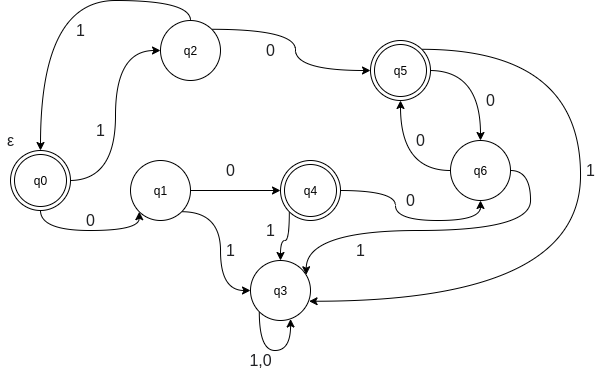
\includegraphics[scale=.70]{firstAFD.png}
                    Metodo usado:
                    Me enfoque en las dos condiciones mas importantes que v\'i, la primera que el numero de unos y ceros
                    sean pares lo cual lo cubr\'i con los estados q0 y q2 para los unos y con q5 y q6 para los ceros.
                    Para asegurarme que despues de un 0 no se puedan agregar unos utilice los estados q1, q4 y q3 donde q3 es un 
                    estado de error para que de ahi ya no pase nada. 
                \end{solution}
        \end{enumerate}
        \question Sea $L_{3} = \{w=a_{0}a_{1}...a_{k} | a_{k-3}=0, k \geq 3\}$ sobre el alfabeto $\Sigma = \{0,1\}$:
        \begin{enumerate}
            \item Diseña un AFN (sin transiciones épsilon) que acepta el lenguaje.
            \begin{solution}
                \\
                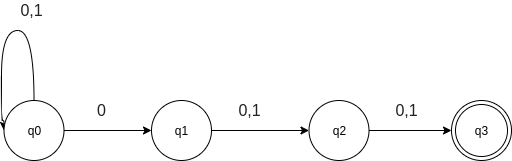
\includegraphics[scale=.70]{last.png}
            \end{solution}
            \item Transforma el AFN anterior a un AFD e incluye la gr\'afica.
        \end{enumerate}
\end{questions}


